\documentclass[conference]{IEEEtran}

\usepackage{amsmath}
\usepackage{amsfonts}
\usepackage{amssymb}
\usepackage{makeidx}
\usepackage{graphicx}
\usepackage{booktabs}
\usepackage{amsmath}
\usepackage{algorithm}

\usepackage[noend]{algpseudocode}
\usepackage{url}

\usepackage{color}

\usepackage{url}

\usepackage{color}

\newcommand{\eat}[1]{}
\newenvironment{definition}[1][Definition]{\begin{trivlist}
\item[\hskip \labelsep {\bfseries #1}]}{\end{trivlist}}

\begin{document}
\author{\IEEEauthorblockN{Anmol Singh Sethi}
\IEEEauthorblockA{IIT2016040}
\and
\IEEEauthorblockN{Anirudh Singh Rathore}
\IEEEauthorblockA{IIT2016091}
\and
\IEEEauthorblockN{Dheeraj Chouhan}
\IEEEauthorblockA{IIT2016078}
\and
\IEEEauthorblockN{Manish Ranjan}
\IEEEauthorblockA{IIT2016059}
\and
\IEEEauthorblockN{Vikas Kumar}
\IEEEauthorblockA{IIT2016058}}

\title{Calculation of Determinant Of An NxN Matrix Using Recursion}
\maketitle
\begin{abstract}
An algorithm involving the calculation of the determinant of a NxN square matrix using recursion. 
\end{abstract}

\begin{IEEEkeywords}
recursion, determinant, square-matrix, time-complexity\end{IEEEkeywords}

\section{Introduction and Literature Survey}
% \begin{figure}[H]   
%   \begin{center}
%     \includegraphics[scale=0.6]{1.JPG} 
%     \caption{Classic Ship Analysis}\label{Saturation}
%   \end{center}
% \end{figure}
The process in which a function calls itself directly or indirectly is called recursion and the corresponding function is called as recursive function. The question involved the calculation of the determinant of matrix using recursion.
Now, we have understood the basic idea of what recursion is. Now let us try to understand a bit about the matrices and their determinants.
\\Determinant of a Matrix is a special number that is defined only for square matrices (matrices which have same number of rows and columns). Determinant is used at many places in calculus and other matrix related algebra, it actually represents the matrix in term of a real number which can be used in solving system of linear equation and finding the inverse of a matrix. The determinant of a matrix A is denoted det(A), det A.
\[
\det(A) =
\begin{vmatrix}
a & b\\ 
c & d\\
\end{vmatrix}
=
\ ad-bc
\]
\\Similarly, suppose we have a 3 × 3 matrix A, and we want the specific formula for its determinant det(A):
\[
\det(A) =
\begin{vmatrix}
a & b & c\\ 
d & e & f\\
g & h & i\\
\end{vmatrix}
=
\ aei + bfg + cdh - ceg - bdi - afg 
\]
Each determinant of a 2 x 2 matrix in calculation of a 3 x 3 matrix equation is called a minor of the matrix A. The same sort of procedure can be used to find the determinant of a 4 x 4 matrix, the determinant of a 5 x 5 matrix, and so forth.
\ Let us take a moment and take a note of an important property for the determinant of the matrix, which is as follows:-
\\ This n-linear function is an alternating form: whenever two rows of a matrix are identical, its determinant is 0.

\section{Algorithm Design And Explanation}
A very simple recursive algorithm has been designed for the purpose stated above. The algorithm has the following steps:-\\
\\1. The base condition for the recursive function is whenever the matrix is containing only one element. In such a case that element is the value of the determinant.
\\2. A variable "det" is taken which stores the value of the determinant and is returned at the ed finally.
\\3. For the first row the minor is computed and it's determinant is multiplied with it, which is calculated recursively by calling the function containing the minor matrix. The temp contains the minor matrix for that function.
\\4. While calculating the minor matrix, the elements in the row and column of the "col" are left and other are put into place by checking the boundary conditions.
\\5. The sign which is one of the multiplying factors in the expression is changed every time the function is called.
\\6. return the determinant for every function and add it to the final result while exiting the recursive calls.
\\ The pseudo-code for the algorithms described above is the following:-\\
\\\textit{Input}: An N x N matrix filled with random numbers.
\\\textit{Output}: A single integer value denoting the determinant of the matrix.
\bigskip
\begin{algorithm}
\caption{To Find Determinant of (n x n) Matrix Using Recursion}\label{basic}
\begin{algorithmic}  
\Procedure{$determinant$}{arr[N][N], n}
\State\textit{$sign\gets1$}
\If{( n=1 )}
	    	\State\textit{$return \ arr[0][0]$}
            
\Else{}  
		\State\textit{$det\gets0$}
  		\For { ( col = 0 to (n-1) } 
        \If{(arr[0][col] = 0 )}
	    	\State\textit{$goto \ label$}
         \EndIf
        \State\textit{$a\gets0$}
        \State\textit{$b\gets0$}
		
         \For{( i = 0 to n-1 )}
    	\For{( j = 0 to n-1 )}
    	\If{( i != 0 \&\& j != col  )}
	    	\State\textit{$temp[a][b++] \gets arr[i][j]$}
            \If{( $b = (n-1) $ )}
	    		\State\textit{$a\gets(a+1)$}
                \State\textit{$b\gets 0 $}
         	\EndIf
         \Else{}
         	\State\textit{$temp[i][j]\gets0$}
         \EndIf
    \EndFor
    \EndFor
    \State\textit{det = det+ sign*(arr[0][col]*determinant(temp, n-1))}
    \State\textit{$label : sign = sign*(-1)$}
\EndFor
    \EndIf
    \State\textit{$return \  det$}
\EndProcedure


\Procedure{$main()$}{}
\For{( i =  0 to (N-1) )}
      \For{( j =  0 to (N-1) )}
          	\State\textit{$scan( arr[i][j])$}
        \EndFor
        \EndFor
\State\textbf{print(determinant(arr, N))}\\
\EndProcedure
\end{algorithmic}
\end{algorithm}

\section{Time Complexity Analysis and Discussion}
Consider the three scenarios:-\\ 
1. \textit {Worst Case }: \\
\ For e.g. 
$$\begin{pmatrix}
1 & 2 & 3\\
4 & 5 & 5\\
8 & 7 & 6\\
\end{pmatrix}$$
2. \textit {Best Case}:-\\
\ For e.g. 
$$\begin{pmatrix}
0 & 0 & 0\\
1 & 3 & 4\\
9 & 7 & 5\\
\end{pmatrix}$$.
3. \textit{ Average Case}:-\\
\ For e.g. 
$$\begin{pmatrix}
1 & 2 & 3\\
4 & 0 & 5\\
8 & 7 & 6\\
\end{pmatrix}$$
\section{Experimental Study}
In this section of the repost the actual data of the time calculation has been shown. The time plots have been constructed using the unit time equations at every step of the computation. Further the data was written in a file and GNU plots were constructed to verify our claims in the previous sections.

\begin{table}[h!]
  \begin{center}
    \caption{Time Complexity Table}
    \label{tab:table1}
    \begin{tabular}{l|l|l|l}
      \textbf{n} & \textbf{t\textsubscript{best}} & \textbf{t\textsubscript{average}} & \textbf{t\textsubscript{worst}}\\ % <-- added & and content for each column
%       $\alpha$ & $\beta$ & $\gamma$ & $\delta$ \\ % <--
      \hline
      2 & 18 & 69 & 120 \\
      3 & 25 & 691 & 691 \\
      4 & 32 & 3504 & 3504 \\
      5 & 39 & 18929 & 18929 \\
      6 & 46 & 63898 & 115978 \\
      7 & 53 & 400743 & 815637 \\
      8 & 60 & 4252328 & 6530732 \\
      9 & 67 & 27009117 & 58784593 \\
      10 & 74 & 309543244 & 587856894 \\
      
%       2 & 10.1 & b & f\\ % <--
%       3 & 23.113231 & c & ]g\\ % <--
    \end{tabular}
  \end{center}
\end{table}


\begin{figure}[H]
  \begin{center}
    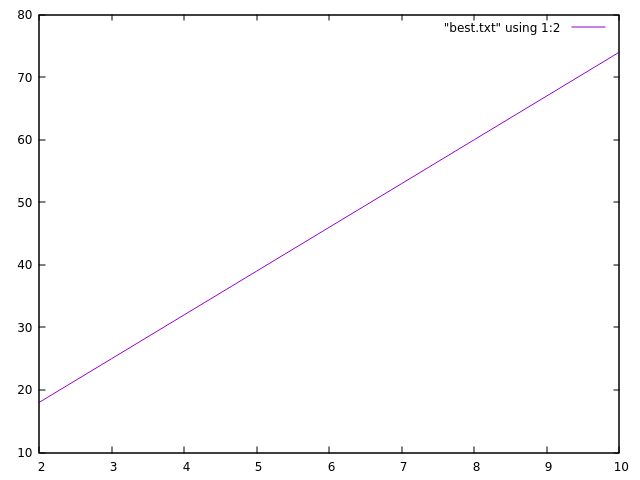
\includegraphics[scale=0.5]{best.png} 
    \caption{Best-Case T(y-axis) VS N(x-axis) }\label{Saturation}
  \end{center}
\end{figure}

\begin{figure}[H]
  \begin{center}
    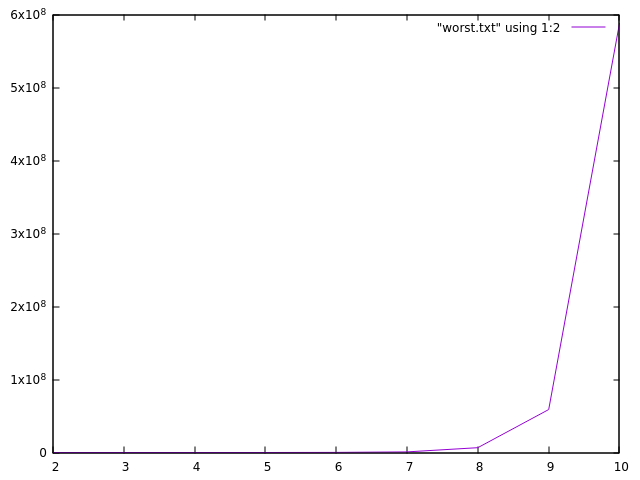
\includegraphics[scale=0.5]{worst.png} 
    \caption{Worst-Case T(y-axis) VS N(x-axis) }\label{Saturation}
  \end{center}
\end{figure}

\begin{figure}[H]
  \begin{center}
    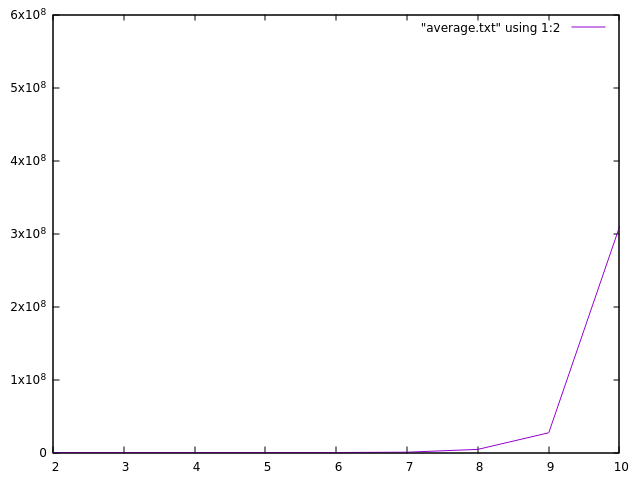
\includegraphics[scale=0.5]{average.png} 
    \caption{Average-Case T(y-axis) VS N(x-axis) }\label{Saturation}
  \end{center}
\end{figure}

\begin{figure}[H]
  \begin{center}
    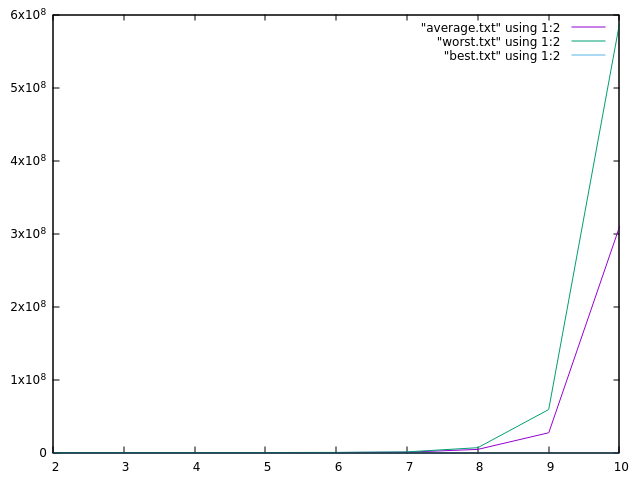
\includegraphics[scale=0.5]{relative.png} 
    \caption{All cases relatively. T(y-axis) VS N(x-axis) }\label{Saturation}
  \end{center}
\end{figure}

\section{Conclusion}
Here, an attempt has been made to find the determinant of the matrix using a recursive approach. The details of the algorithms have been also discussed and experimental analysis of the designed algorithms was carried out.Moreover, all the possible cases have been discussed for the formation of as efficient algorithm as possible.

\begin{thebibliography}{99}

\bibitem{c1}http://www.hec.ca/en/cam/help/topics/Matrixdeterminants.pdf\\
\bibitem{c1} https://en.wikipedia.org/wiki/Determinant\\
\bibitem{c1}https://www.geeksforgeeks.org/recursion/\\
\bibitem{c1}https://www.geeksforgeeks.org/determinant-of-a-matrix/\\
\bibitem{c1}
http://www.maths.surrey.ac.uk/explore/emmaspages/option1.html
\\





\end{thebibliography}

\end{document}

